\begin{surferPage}{Um Cone Duplo}
   Como vimos na introdu\c c\~ao desta galeria, uma superf\'icie diz-se 
    \emph{n\~ao--singular} ou suave se ela n\~ao tiver nenhum v\'ertice
   (tais pontos s\~ao chamados {\it singularidades}).
    Por exemplo, uma superf\'icie esf\'erica ou um toro (as duas imagens abaixo mais \`a esquerda):
    \begin{center}
      \vspace{-0.3cm}
      \begin{tabular}{@{}c@{}c@{}c@{}c@{}}
        \begin{tabular}{@{}c}
          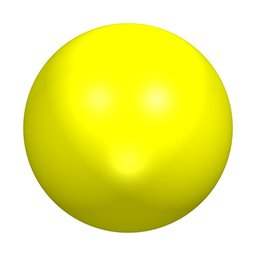
\includegraphics[width=1.4cm]{./../../common/images/kugel}
        \end{tabular}
        &
        \begin{tabular}{@{}c}
          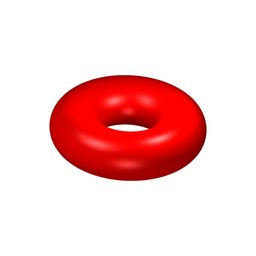
\includegraphics[width=1.4cm]{./../../common/images/torus}
        \end{tabular}
        &
        \begin{tabular}{c@{}}
          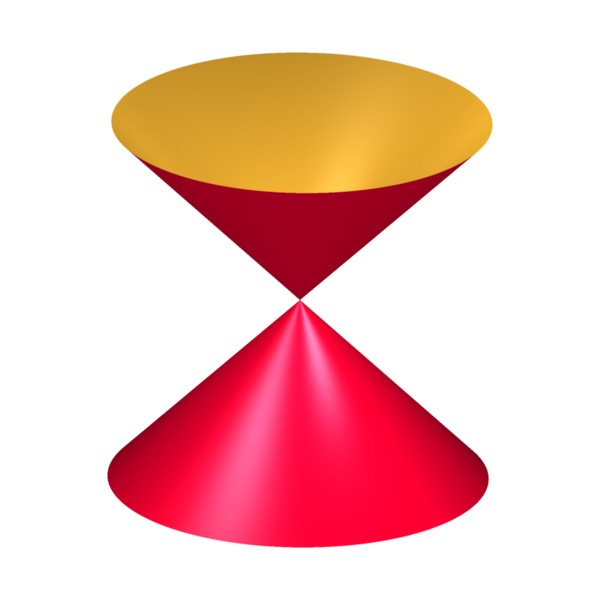
\includegraphics[width=1.4cm]{./../../common/images/kegel}
        \end{tabular}
      \end{tabular}
    \end{center}
    \vspace{-0.3cm}
     O cone duplo (imagem mais \`a direita) \'e a singularidade mais simples; ela \'e a \'unica singularidade que pode ser descrita por uma equa\c c\~ao de grau $2$:
    \[x^2+y^2-z^2=0.\]
    Modificando um pouco essa equa\c c\~ao, substitu\'indo o $0$ por um valor pequeno
    $a\neq 0$, o cone duplo transforma-se em dois tipos de hiperboloides, dependendo do sinal de $a$:

%    \dontshow{
    % 
    \begin{center}
      \vspace{-0.2cm}
      \begin{tabular}{@{}c@{\ }c@{\ }c@{\ }c@{\ }c@{}}
        \begin{tabular}{@{}c@{}}
          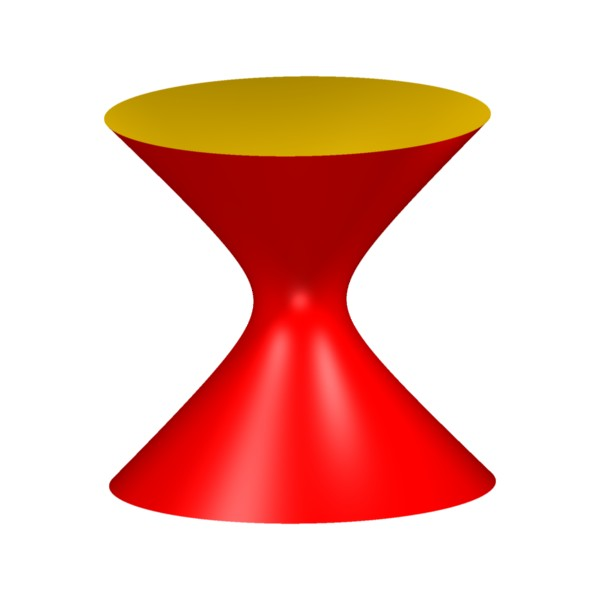
\includegraphics[width=1.2cm]{./../../common/images/A1pm_2}
        \end{tabular}
        &
        $\leftarrow$
        &
        \begin{tabular}{@{}c@{}}
          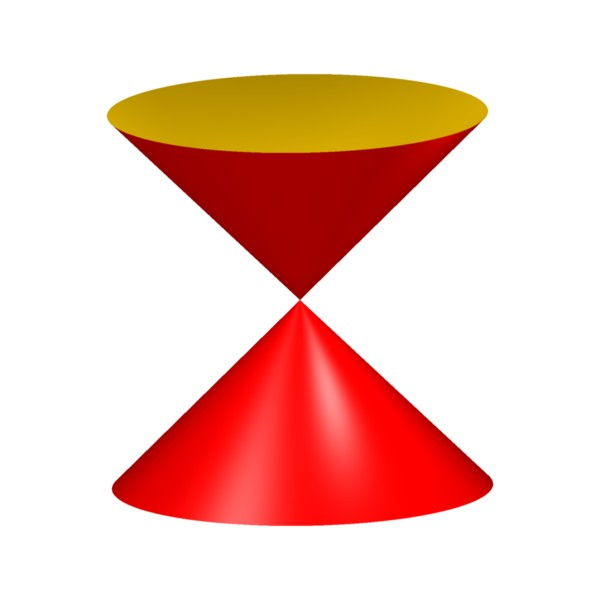
\includegraphics[width=1.2cm]{./../../common/images/A1pm_1} 
        \end{tabular}
        &
        $\rightarrow$
        &
        \begin{tabular}{@{}c@{}}
          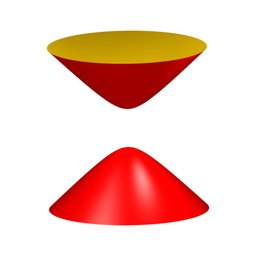
\includegraphics[width=1.2cm]{./../../common/images/A1pm_0}
        \end{tabular}
      \end{tabular}
    \end{center}
%    }
    \vspace{-0.2cm}
   Uma superf\'icie de grau $2$ n\~ao pode ter mais do que uma singularidade, ou seja, \  
    $\mu(2)=1$.
\end{surferPage}
